%%%%%%%%%%%%%%%%%%%%%%%%%%%%%%%%%%%%%%%%%%%%
\section{Content Delivery: The Landscape}\label{sec:content-delivery}
%%%%%%%%%%%%%%%%%%%%%%%%%%%%%%%%%%%%%%%%%%%%

Internet traffic grows at a rate of approximately 30\% per
year~\cite{cisco-study} and is dominated by the delivery of content to end
users~\cite{IXPSIGCOMM2012,TrafficTypesGrowth:2011,arbor,PADIS2010}. To cope
with the increasing demand for content, and to support the level of reliability
and scalability required by commercial-grade applications, Content Distribution
Infrastructures (CDIs) have emerged. In general terms, CDIs are overlays built
on top of existing network infrastructures that aim to accelerate the delivery
of content to end-users. CDIs include, but are not limited to, Content
Distribution Networks (CDNs), such as Akamai and Google, Video Streaming
Portals (VSP) such as YouTube, One-Click-Hosters (OCH) like Rapidshare and
MegaUpload. However, a CDI does not necessarily produce the content that it
delivers. Thus, we define a Content Producer (CP) as the entity that generates
content. In some cases, \eg Google and YouTube, the CP and CDI can be the same
entity. In other instances, for example Akamai and Limelight, the CDI only
delivers what a CP pays for.

But not all CDIs are built upon the same philosophy, designs and technology.
For example, a CDI can be operated independently by deploying caches in
different networks, by renting space in datacenters or by building its own
datacenters. Furthermore, some CDIs are operated by ISPs, by Content Producers,
or in the case of Peer-to-Peer networks, by self-organized end-users. To
summarize the spectrum of CDI solutions, Figure~\ref{fig:cdn-spectrum} provides
an overview of different CDI solutions. They are aligned by their architectures
according to which parties are involved.

\begin{figure}[tbp]
    \begin{center}
    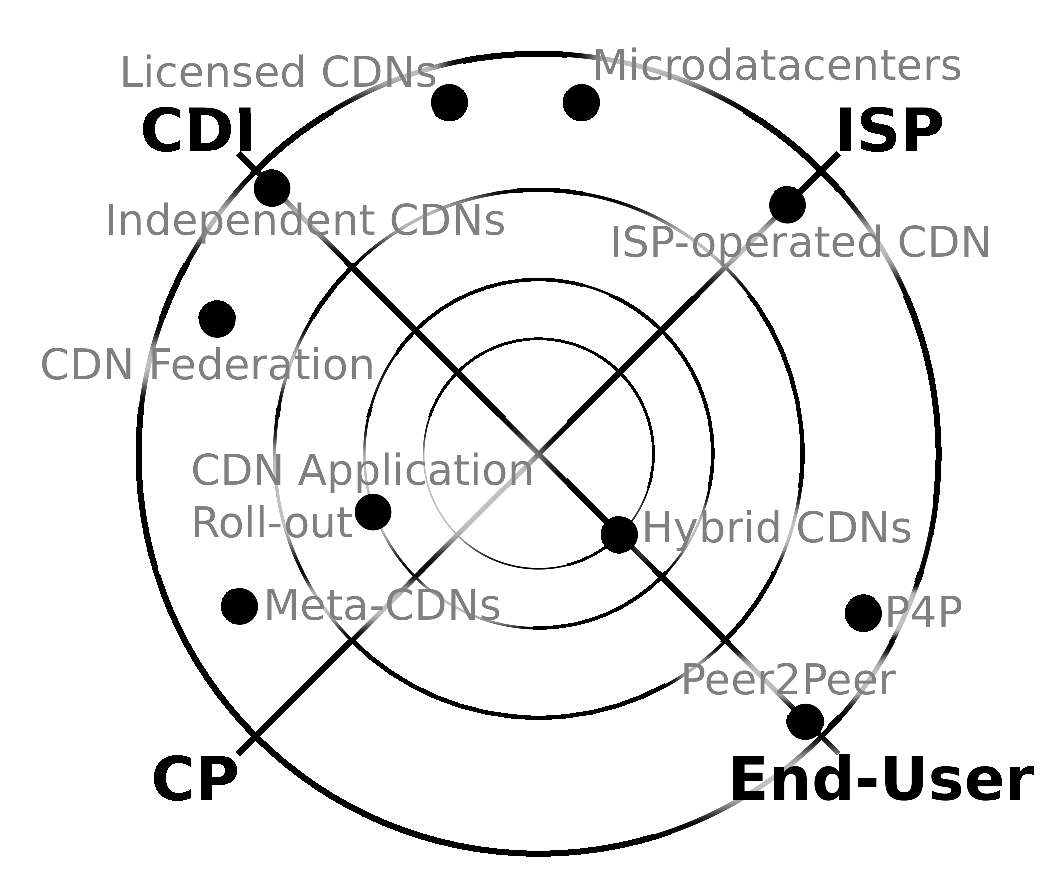
\includegraphics[width=0.7\linewidth]{figures-pdf/spectrum}
    \end{center}
    \caption{Spectrum of content delivery solutions and involvement of
      stake-holders in the content delivery. Reprinted from
      \cite{NetPaaS}. Included here by permission.}
    \label{fig:cdn-spectrum}
\end{figure}

\subsection{Independent Content Distribution}

Independent CDIs are usually referred to as Content Delivery Networks (CDNs).
They have a strong customer base of content producers and are responsible for
delivering the content of their customers to end-users around the world.
Today, they are, by traffic volume as well as hosted content, the largest
players on the Internet. In general, there are four main components to
independent CDN architectures: a server deployment, a strategy for replicating
content on servers, a mechanism for directing users to servers, and a system
for collecting and processing server logs.

For server deployment, three main approaches
exist~\cite{ImprovingPerformanceInternet2009}: centralized, datacenter based
and distributed infrastructures:

\textbf{Central Location}: This approach is used by small CDNs, One-Click
Hosters, and applications running in public clouds. Centralized hosting takes
advantage of (a) the economies of scale that a single location offers~
\cite{aboveclouds}, (b) the flexibility that multihoming
offers~\cite{Optimizing:Goldenberg2004}, and (c) the connectivity opportunities
that IXPs offer~\cite{IXPSIGCOMM2012}. The disadvantages of centralized hosting
are the potential for a single point of failure, and the limited ability to
ensure low latency to users located in different networks around the
world~\cite {CloudCmp}.

\textbf{Datacenter Based}: This approach deploys in several large data centers.
It again leverages economies of scale while improving reliability and creating
a larger footprint with further reach. However, by utilizing multiple
datacenters, new challenges regarding the content distribution, synchronization
and delivery arise. For example, the datacenter delivering content to an
end-user cannot be statically configured anymore, but the selection needs to
take the location of the end-user into account. This approach is used by CDNs
such as Limelight, EdgeCast and BitGravity. Many cloud providers also use this
approach, including Amazon CloudFront and Microsoft Azure.

\textbf{Distributed Infrastructures}: This approach consists of a highly
distributed infrastructure deployment, potentially deep inside third-party
networks. Here, the large number of servers scattered across numerous networks
offer high availability and replication of content while being very close to
end-users. Furthermore, this type can balance traffic across locations, best
react to flash crowds by dynamic server assignments, and deliver content with
improved latency. However, with the highly distributed infrastructures, the
challenges of assigning users to the right server location increase many-fold.
Also, with deep deployment datacenters are usually not available anymore,
leading to the question where to deploy how many servers. Today, Akamai is only
one independent CDN that uses this approach on a global scale.

\vspace{0.5em} CDNs with more than one location typically follow a pull
strategy~\cite{Akamai-Network} for content distribution and replication. Thus,
content requests can be directed to servers that do not have the required
object cached.  When a requested object is not at the selected server,
neighboring servers in the same cluster or region are asked. If the object is
not available at neighboring servers, the origin or root server responsible for
the object is contacted to retrieve the content. A requested object that is
fetched from a remote server is saved locally and then delivered to the end
user. To keep the copies of the object fresh, a TTL value is assigned to it.
When the TTL value expires, the object is removed. For scalability reasons, any
server of the CDN or within a region can respond to the request of an end
user~\cite{CDNsec2009}.

A special case of the independent CDI category are free CDNs such as
Coral~\cite{CoralCDN}, which follow a similar architectural design. In these
CDNs, server resources are offered by end-users or non-profit organizations.

\subsection{ISP-operated CDIs} The potential for generating revenue from
content delivery has motivated a number of ISPs to build and operate their own
Content Distribution Infrastructures. For example, large ISPs such as AT\&T and
Verizon have built their own CDNs along the same general architectural
principles as independent CDIs. However, due to the limitations arising from
being restricted to one network, these CDNs are not deployed in a distributed
fashion across multiple networks and thus are not globally operating solutions.
To overcome this issue, the CDNi group at the IETF~\cite {CDNi} is discussing
how to interconnect these CDNs to boost their efficiency and coverage. The
content provider are third parties, applications and services offered by the
ISP. Other ISPs with large footprints, such as Level3 and Telefonica~ \cite
{interdatacenter,ToN-DTB}, have also built CDNs in order to efficiently
transfer content across the globe and offer improved services to their end
users.

\subsection{Emerging Trends in CDI Architectures} Economics, especially cost
reduction, is the key driving force behind emerging CDI architectures. The
content delivery market has become highly competitive. While the demand for
content delivery services is rising and the cost of bandwidth is decreasing,
the profit margins of storage and processing \cite{aboveclouds} are dwindling,
increasing the pressure on CDIs to reduce costs. At the same time, more parties
are entering the market in new ways, looking to capture a slice of the revenue.
However, today's traditional CDI deployments lack agility to combat these
effects.  Contracts for server deployments last for months or years and the
available locations are typically limited to datacenters. The time required to
install a new server today is in the order of weeks or months. Such timescales
are too large to react to changes in demand. CDIs are therefore looking for new
ways to expand or shrink their capacity, on demand, and especially at low cost.

\subsubsection{Hybrid Content Distribution} In a hybrid CDI, end-users download
client software that assists with content distribution. As in P2P file-sharing
systems, the content is broken into pieces and offered by both other users who
have installed the client software as well as by the CDI's servers. The client
software contacts dedicated CDI servers, called control plane servers, which
schedule which parts of the content are to be downloaded from what peers.
Criteria for selecting peers include AS-level proximity as well as the
availability of the content. If no close peers are found, or if the download
process from other peers significantly slows the content delivery process, the
traditional CDI servers take over the content delivery job entirely. Akamai
already offers NetSession~\cite{HybridCDN-Bruce}, a hybrid CDI solution for
delivering very large files such as software updates at lower cost to its
customers.  Xunlei~\cite{Xunlei}, an application aggregator with high
penetration in China, follows a similar paradigm.  It is used to download
various types of files including videos, executables, and even emails, and
supports popular protocols such as HTTP, FTP, and RTSP.  Xunlei maintains its
own trackers and servers. A study of hybrid CDIs~\cite{HybridCDN-Ross} showed
that up to 80\% of content delivery traffic can be outsourced from server-based
delivery to end-users, without significant degradation in total download time.

\subsubsection{Licensed CDNs} Licensed CDNs have been proposed to combine the
benefits of the large content-provider customer base of an independent CDI with
the end-user base of an ISP~\cite{LicensedCDN}.  A licensed CDN is a
partnership between an independent CDI and an ISP. The CDI licenses the content
delivery software that runs on servers to the ISP while the ISP owns and
operates the servers. The servers deliver content to the end-users and report
logging information back to the CDI.  The revenue derived from content
producers is then shared between the two parties. Thus, a CDI can expand its
footprint deep inside an ISP network without investing in hardware, incurring
lower operating costs.  The ISP benefits from not having to invest in
developing the software for a reliable and scalable content distribution. More
importantly, a licensed CDN also alleviates the ISP's need to negotiate
directly with content producers, which might be challenging, given an ISPs
limited footprint.

\subsubsection{Application-based CDIs} Recently, large application and content
producers have rolled out their own CDIs, hosted in multiple large data
centers. Some popular applications generate so much traffic that the content
producers can better amortize delivery costs by doing content distribution
themselves.  Google is one such example.  It has deployed a number of data
centers and interconnected them with high speed backbone networks.  Google
connects its datacenters to a large number of ISPs via IXPs and also via
private peering.  Google has also launched the Google Global Cache
(GGC)~\cite{GoogleCache}, which can be installed inside ISP networks.  The GGC
reduces the transit cost of small ISPs and those that are located in areas with
limited connectivity, \eg Africa. The GGC servers are given for free to the
ISPs which install and maintain them.  GGC also allows an ISP to advertise
through BGP the prefixes of users that each GGC server should serve.  As
another example, Netflix, which is responsible for around 30\% of the traffic
in North America at certain times, is also rolling out its own CDI. The Netflix
system is called Open Connect Network~\cite{NetflixCDN}. Netflix offers an
interface where ISPs can advertise, via BGP, their preferences as to which
subnets are served by which Open Connect Network servers.

\subsubsection{Meta-CDIs} Today, content producers contract with multiple CDIs
to deliver their content.  To optimize for cost and
performance~\cite{Optimizing:SIGCOMM2012}, meta-CDIs act as brokers to help
with CDI selection. These brokers collect performance metrics from a number of
end-users and try to estimate the best CDI, based on the server that a user is
assigned. To this end, the brokers place a small file on a number of CDIs. Then
they embed the request for this file in popular websites' source code, in the
form of a javascript. When users visit these sites, they report back statistics
based on the servers that each CDI assigned the users. The broker then
recommends CDIs for a given source of demand taking also into consideration the
cost of delivery. Cedexis is one of these brokers for web browsing.  Another
broker for video streaming is Conviva~\cite{Conviva2011}. These brokers may
compensate when a CDI does not assign a user to the optimal server (which a
recent study~\cite{PADIS2010} has shown sometimes occurs) by selecting a
different CDI.


\subsubsection{CDI Federations} To avoid the cost of providing a global
footprint and perhaps to allow for a single negotiating unit with content
providers, federations of CDIs have been proposed. In this architecture,
smaller CDIs, perhaps operated by ISPs, join together to form a larger
federated CDI.  A CDI belonging to the federation can replicate content to a
partner CDI in a location where it has no footprint.  The CDI reduces its
transit costs because it only has to send the object once to satisfy the demand
for users in that location. Overall, cost may be reduced due to distance-based
pricing~\cite{HowManyTiers}. The IETF CDNi working group \cite{CDNi} works on
CDI federation.

